\documentclass[10pt]{article}

\usepackage{times}
\usepackage{hyperref}
\usepackage{float}

\textwidth=6.5in
\textheight=8.5in
\oddsidemargin=-.1in
\evensidemargin=-.1in
\headheight=-.3in

\newcommand{\Rfunction}[1]{{\texttt{#1}}}
\newcommand{\Robject}[1]{{\texttt{#1}}}
\newcommand{\Rpackage}[1]{{\textit{#1}}}
\newcommand{\Rmethod}[1]{{\texttt{#1}}}
\newcommand{\Rfunarg}[1]{{\texttt{#1}}}
\newcommand{\Rclass}[1]{{\textit{#1}}}
\newcommand{\Rcode}[1]{{\texttt{#1}}}
\newcommand{\software}[1]{\textsf{#1}}
\newcommand{\R}{\software{R}}
\newcommand{\predictiveModeling}{\Rpackage{predictiveModeling}}
\newcommand{\synapseClient}{\Rpackage{synapseClient}}

\title{Building predictive models of drug sensitivity using Synapse}
\author{Adam Margolin, Nicole Deflaux}
\date{\today}



\usepackage{Sweave}
\begin{document}

\maketitle

\section{Sage Bionetworks Synapse project}

The recent exponential growth of biological ``omics'' data has occurred
concurrently with a decline in the number of NMEs approved by the FDA. Sage
Bionetworks believes that a fundamental reason biological research
productivity does not scale with biological data generation is that the
analysis and interpretation of genomic data remains largely an isolated,
individual activity. Sage Bionetworks' mission is to catalyze a cultural
transition from the traditional single lab, single-company, and
single-therapy R\&D paradigm to a model with broad precompetitive
collaboration on the analysis of large scale data in medical sciences. For
this to happen it is critical that: 1) human health data become accessible
and reusable by people other than the original data generators allowing
multiple parallel approaches to data interpretation; 2) analytical
methodologies become fully reproducible and transparent so that results can
be vetted and existing analysis techniques quickly applied to new
application areas, and; 3) models of biological systems and networks be
opened to a variety of users such that theoretical predictions can be
rapidly validated experimentally and improve standards of care for
patients. Sage Bionetworks is actively engaged with academic and
pharmaceutical collaborators in developing technical, policy and strategic
solutions to these issues. Part of Sage's solution is Synapse, a platform
for open, reproducible data-driven science, which will provide support for
Sage's research initiatives and serve as a resource for the broader
scientific community.

Synapse will support the reusability of information facilitated by
ontology-based services and applications directed at scientific researchers
and data curators. Sage Bionetworks is actively pursuing the acquisition,
curation, statistical quality control, and hosting of human and mouse global
coherent datasets for use by Sage Bionetworks researchers, collaborators,
and the broader research community. Global coherent datasets integrate both
clinical phenotype and genomic data along with an intermediate molecular
layer such as gene expression or proteomic data. Typically studies contain
genome-wide genetic variation data and/or expression profiling data. We
expect the release of these sorts of unique, integrative, high value
datasets into the public domain will seed a variety of analytical approaches
to drive new treatments based on better understanding of disease states and
the biological effects of existing drugs.

Reproducible analysis and disease model reuse require a supporting
informatics infrastructure. In the Sage Bionetworks system, users interact
with resources via a number of mechanisms depending upon their interests and
expertise. The Synapse web portal will be an environment for end user
scientists to interact and share data, models, and analysis methods, both in
the context of specific research projects, and broadly across otherwise
disparate projects. Many other specialized scientific tools can be extended
to load data and save results to the Sage Bionetworks platform, or to
perform analysis by calling methods executed on a remote service. The Sage
Bionetworks Platform is aggressively leveraging and optimizing its
architecture to take full advantage of the rapidly maturing cloud computing
technologies which will put on-demand supercomputing power in the hands of
the average researcher.  These more specialized analytical clients would
support use cases in data curation and quality control as well as scientific
analysis.

\section{Set up your Synapse work environment}

Go to \url{https://synapse-alpha.sagebase.org/} to register for a new
account and then log into Synapse.

\begin{figure}[H]
  \centering
  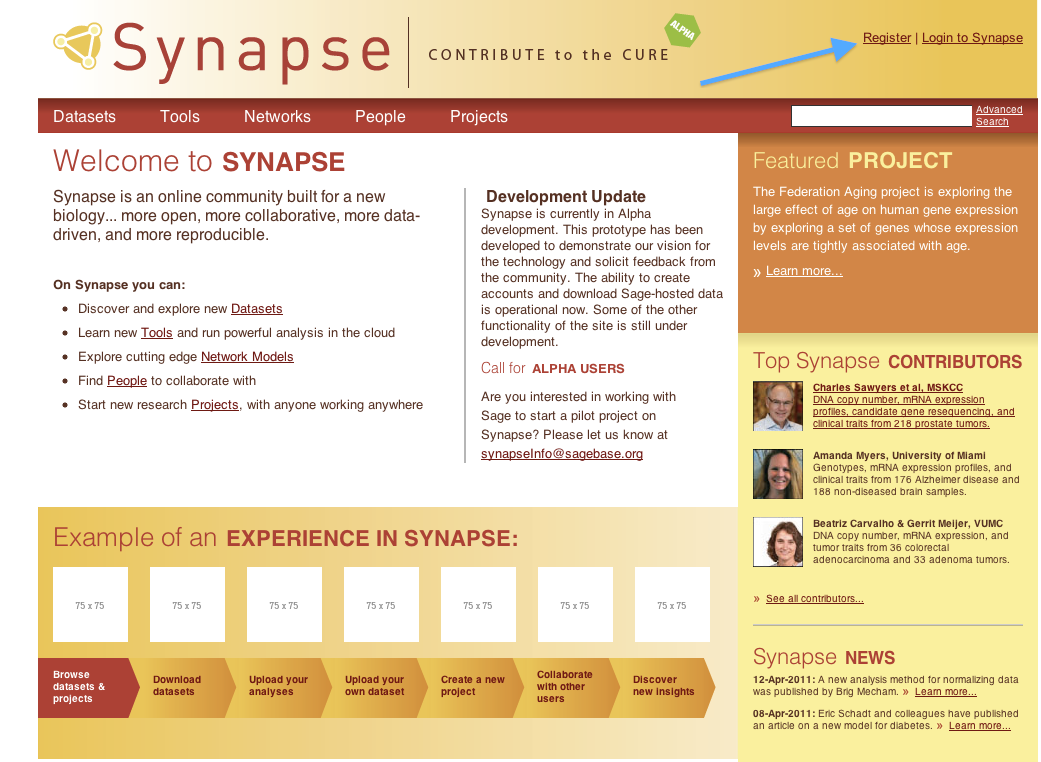
\includegraphics{synapseScreenshots/Register.png}
  \caption{Register for a Synapse account and log in}
\end{figure}

Use the following R code to setup your Synapse work environment.

\begin{Schunk}
\begin{Sinput}
> library(predictiveModeling)
\end{Sinput}
\begin{Soutput}
randomSurvivalForest 3.6.3

Type rsf.news() to see new features, changes, and bug fixes.
\end{Soutput}
\begin{Sinput}
> # Change the values of these variables 
> myName <- Sys.getenv("USER")
> myWorkingDirectory <- "."
> setwd(myWorkingDirectory)
\end{Sinput}
\end{Schunk}

Create a Synapse project to hold your analyses results.  Be sure to type in
your Synapse username and password when prompted from R.

\begin{Schunk}
\begin{Sinput}
> library(synapseClient)
> synapseLogin()
> project <- Project(list(
+   name=paste("Machine Learning Results - ", myName)
+   ))
> project <- createEntity(project)
> onWeb(project)
> analysis <- Analysis(list(
+     name="Elastic net versus custom methods",
+     description="Several Machine Learning methods run upon CCLE Data with Sanger Drug Response",
+     parentId=propertyValue(project, "id")
+     ))
> analysis <- createEntity(analysis)
> dataset <- Dataset(list(
+   name="Analysis Plots",
+   parentId=propertyValue(project, "id")
+   ))
> dataset <- createEntity(dataset)
\end{Sinput}
\end{Schunk}

Go back to \url{https://synapse-alpha.sagebase.org/} and find your newly created
project.  Click on ``share'' and share your project with the group
AUTHENTICATED\_USERS.

\begin{figure}[H]
  \centering
  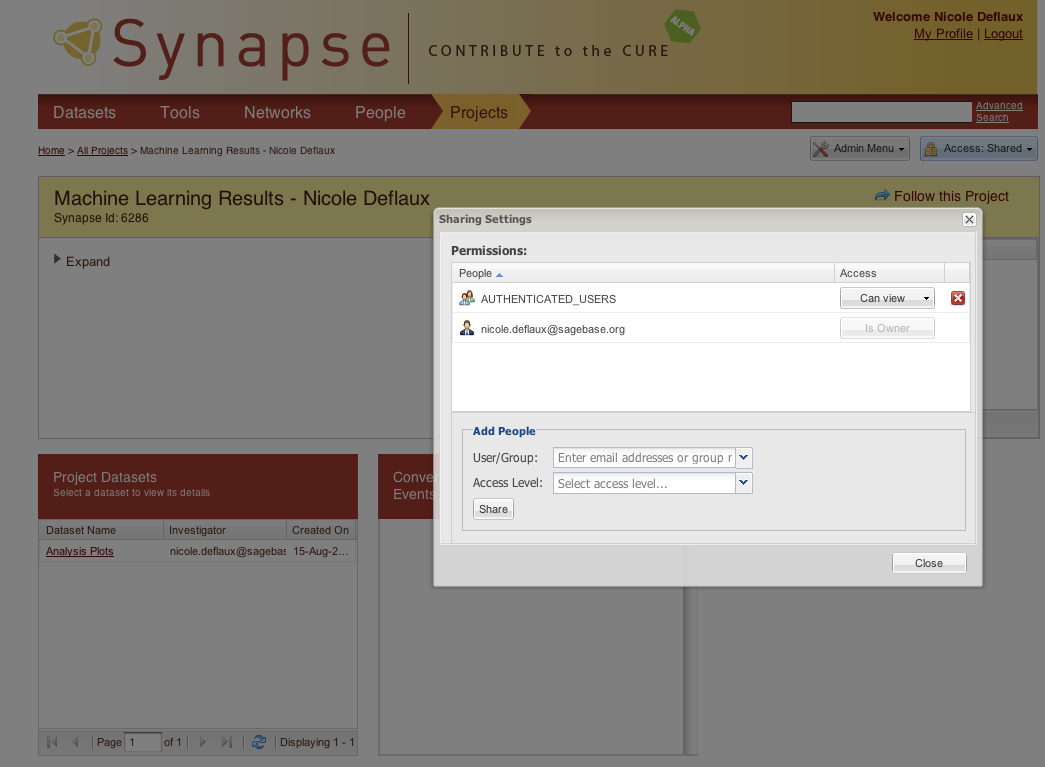
\includegraphics{synapseScreenshots/Sharing.png}
  \caption{Find your project and share it with AUTHENTICATED\_USERS}
\end{figure}

\section{Load data from Synapse}

Navigate to the ``Cell Line Project'' in Synapse
\url{https://synapse-alpha.sagebase.org/#Project:5019}.  Click on the two
datasets listed there and their layers to get the IDs of the data layers for
CCLE expression, CCLE copy number, CCLE oncomap, and Sanger drug response IC50s.  Note
that you can also browse data available in Synapse via the Synapse R Client.
See the help documentation for synapseClient for more detail.

\begin{figure}[H]
  \centering
  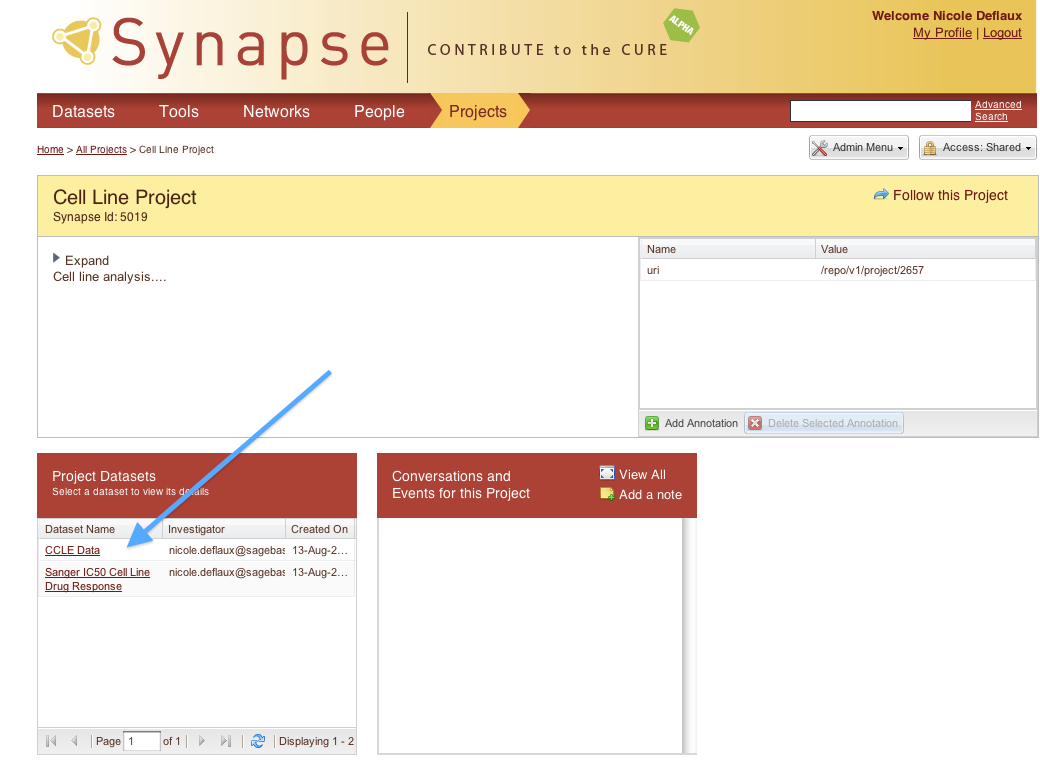
\includegraphics{synapseScreenshots/Datasets.png}
  \caption{Find the CCLE and Sanger Dataset Layers in Synapse}
\end{figure}
  
\begin{Schunk}
\begin{Sinput}
> #### Load Data from Synapse ####
> idExpressionLayer <- "48344"
> expressionLayer <- loadEntity(idExpressionLayer)
> exprSet <- expressionLayer$objects$exprSet
> idCopyLayer <- "48339"
> copyLayer <- loadEntity(idCopyLayer)
> copySet <- copyLayer$objects$copySet
> idOncomapLayer <- "48341"
> oncomapLayer <- loadEntity(idOncomapLayer)
> oncomapSet <- oncomapLayer$objects$oncomapSet
> idSangerLayer <- "48337"
> sangerLayer <- loadEntity(idSangerLayer)
> sangerADF <- sangerLayer$objects$sangerADF
\end{Sinput}
\end{Schunk}


\begin{Schunk}
\begin{Sinput}
> print(colnames(pData(sangerADF)))